%%%%%%%%%%%%%%%%%%%%%%%%%%%%%%%%%%%%%%%%%%%%%%%%%%%%%%%%%%
\chapter{Dependent Sources}
This chapter introduces dependant sources: current or voltage sources that depend on other voltage or current levels elsewhere in the network.\\
\\
The idea of a dependent source isn't too far fetched. Consider the mechanical system shown in Figure~\ref{F:5MDS}. Because motor M2's power depends on the position of object A, it acts like a dependent source.

\begin{figure}[H]
\begin{center}
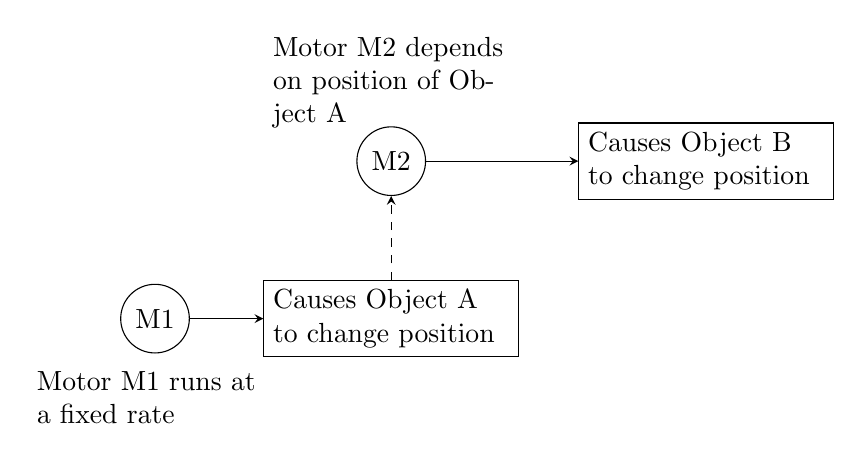
\begin{tikzpicture}
\node [circle, draw=black, fill=white](M1) at (0,0){M1};
\node [rectangle, draw=black, fill=white, text width=3 cm](P1) at (3,0){Causes Object A to change position};
\node [rectangle, draw=black, fill=white, text width=3 cm](P2) at (7,2){Causes Object B to change position};
\node [circle, draw=black, fill=white](M2) at (3,2){M2};
\draw [-stealth](M1) edge (P1);
\draw [-stealth, dashed](P1) edge (M2);
\draw [-stealth](M2) edge (P2);
\draw node at (0,-1) [text width=3 cm] {Motor M1 runs at a fixed rate};
\draw node at (3,3) [text width=3 cm] {Motor M2 depends on position of Object A};
\end{tikzpicture}
\caption{Mechanical System. Motor M2 is a dependent source. Motor M1 is an independent source.}
\label{F:5MDS}
\end{center}
\end{figure}

\noindent
Consider a guitar amplifier for an electrical example. The guitar's \emph{pickup} produces very small voltages and currents. A second voltage source then activates based on the small signals coming from the pickup. The speaker is then powered by the second voltage source.\\

\section{Basic Types}
We have four electrical versions of dependant sources:
\begin{itemize}
\item A voltage source that depends on some other voltage (voltage controlled voltage source, VCVS)
\item A voltage source that depends on some other current (current controlled voltage source, CCVS)
\item A voltage source that depends on some other voltage (voltage controlled current source, VCCS)
\item A voltage source that depends on some other current (current controlled current source, CCCS)
\end{itemize}

Think of these in a table:
\begin{tabular}{|c|c|c|}\hline
$\downarrow$ control \textbackslash out $\rightarrow$ &voltage out&current out \\ \hline
voltage control&vcvs&vccs \\ \hline
current control&ccvs&cccs \\ \hline
\end{tabular}

\begin{figure}[H]
\begin{center}
\begin{tikzpicture}
\draw (0,0)--(0,1)node[diamond, draw=black, fill=white]{$\uparrow$}--(0,2);
\draw node at (-.75,1) {$3V_1$};
\draw node at (0,-.5) {vccs};
\draw (2,0)--(2,1)node[diamond, draw=black, fill=white]{$\uparrow$}--(2,2);
\draw node at (1.25,1) {$3I_1$};
\draw node at (2,-.5) {cccs};
\draw (4,0)--(4,1)node[diamond, draw=black, fill=white, minimum height=1cm, minimum width=1cm]{}--(4,2);
\draw node at (3.25,1) {$3I_1$};
\draw node at (4,1) {$\begin{matrix}+\\-\end{matrix}$};
\draw node at (4,-.5) {ccvs};
\draw (6,0)--(6,1)node[diamond, draw=black, fill=white,minimum height=1cm, minimum width=1cm]{}--(6,2);
\draw node at (5.25,1) {$3V_1$};
\draw node at (6,1) {$\begin{matrix}+\\-\end{matrix}$};
\draw node at (6,-.5) {vcvs};
\end{tikzpicture}
\caption{Four types of dependent sources and their symbols.}
\end{center}
\end{figure}


We will deal only with linear sources, so you won't need to worry about a dependancy like $V=3I_1^2$ in this course \footnote{MOS transistors have non-linear I-V relationships.}.

\subsection{Example 1. Power Amplification}
Consider circuit with a dependent source shown in Figure~\ref{F:5DS}. \footnote{Don't worry yet about how we actually build these dependent sources (we use transistors). Building ANY voltage source requires some doing.}

\begin{figure}[H]
\begin{center}
\begin{tikzpicture}
\draw node at (-1,1) {9V};
\draw (0,0)--(0,1)node[circle, draw=black, fill=white]{$\begin{matrix}+\\-\end{matrix}$}--(0,2)--
(1,2)--(1.1,2.1)--(1.2,1.9)--(1.3,2)--
(2,2)--(2,1)--(1.9,.9)--(2.1,.8)--(2,.7)--(2,0)--(0,0);
\draw (2,0)--(4,0)--(4,1)node[diamond, draw=black, fill=white]{\tiny{$\begin{matrix}+\\-\end{matrix}$}}--(4,2)
--(6,2)--(6,1)--(5.9,.9)--(6.1,.8)--(6,.7)--(6,0)--(4,0);
\draw node at (4.75,1) {$V_1$};
\draw node at (1.25,2.5) {$1k\Omega$};
\draw node at (2.5,1) {$2k\Omega$};
\draw node at (6.5,1) {$10 \Omega$};
\draw node at (1.5,1.5) {+};
\draw node at (1.25,1) {$V_1$};
\draw node at (1.5,.5) {-};
\filldraw (2,2) circle[radius=1 mm];
\node at (2,2.25) {A};
\filldraw (2,0) circle[radius=1 mm];
\node at (2,-.5) {B};
\filldraw (4,2) circle[radius=1 mm];
\node at (4,2.25) {C};
\filldraw (4,0) circle[radius=1 mm];
\node at (4,-.5) {D};
\end{tikzpicture}
\caption{A circuit with a dependent source.}
\label{F:5DS}
\end{center}
\end{figure}

This dependent source forces the voltage from C to D to match the voltage from A to B. It may be surprising that this can have a huge impact on the power absorbed by the $10 \Omega$ resistor, compared with just connecting the 10 Ohm resistor directly to points A and B like shown in Figure~\ref{F:5DS2}.

\begin{figure}[H]
\begin{center}
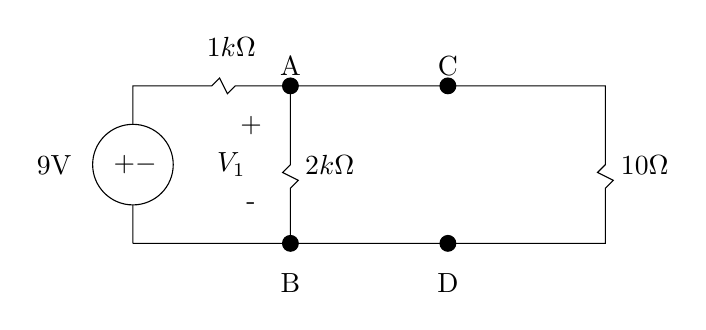
\begin{tikzpicture}
\draw node at (-1,1) {9V};
\draw (0,0)--(0,1)node[circle, draw=black, fill=white]{$\begin{matrix}+\\-\end{matrix}$}--(0,2)--
(1,2)--(1.1,2.1)--(1.2,1.9)--(1.3,2)--
(2,2)--(2,1)--(1.9,.9)--(2.1,.8)--(2,.7)--(2,0)--(0,0);
\draw (2,0)--(4,0) (2,2)--(4,2)
--(6,2)--(6,1)--(5.9,.9)--(6.1,.8)--(6,.7)--(6,0)--(4,0);
\draw node at (1.25,2.5) {$1k\Omega$};
\draw node at (2.5,1) {$2k\Omega$};
\draw node at (6.5,1) {$10 \Omega$};
\draw node at (1.5,1.5) {+};
\draw node at (1.25,1) {$V_1$};
\draw node at (1.5,.5) {-};
\filldraw (2,2) circle[radius=1 mm];
\node at (2,2.25) {A};
\filldraw (2,0) circle[radius=1 mm];
\node at (2,-.5) {B};
\filldraw (4,2) circle[radius=1 mm];
\node at (4,2.25) {C};
\filldraw (4,0) circle[radius=1 mm];
\node at (4,-.5) {D};
\end{tikzpicture}
\caption{Without dependent source. Nodes C and D are no longer useful.}
\label{F:5DS2}
\end{center}
\end{figure}

\begin{clevel}
Fill in the Table~\ref{T:5DS}.
\end{clevel}

\begin{table}[H]
\begin{center}
\begin{tabular}{|c|c|c|} \hline
item&with dependent source&if $10\Omega$ were connected directly to AB \\ \hline
$V_1$&& \\ \hline
$V_{10\Omega}$&& \\ \hline
$I_{10\Omega}$&& \\ \hline
$P_{10\Omega}$&& \\ \hline
\end{tabular}
\caption{Comparison between circuit with and without dependant source.}
\label{T:5DS}
\end{center}
\end{table}

%%%%%%%%%%%%%%%%%%%%%%%%%%%%
\subsection{Example 2. Simple Loop Analysis}
Let's study the dependent source example shown in Figure~\ref{F:5DSb}.

\begin{figure}[H]
\begin{center}
\begin{tikzpicture}
\draw (0,0)--(0,1)node[circle, draw=black, fill=white]{$ \overset{+}{\underset{-}{9V} }$}--(0,2)--
(1,2)--(1.1,2.1)--(1.2,1.9)--(1.3,2)--(2,2)
--(2,1)node[diamond, draw=black, fill=white]{$\downarrow$}
--(2,0)--(0,0);
\draw node at (1,1.6) {$1k\Omega$};
\draw node at (3,1) {$3V_1$};
\draw node at (.5,2.5) {+};
\draw node at (1,2.5) {$V_1$};
\draw node at (1.5,2.5) {-};
\end{tikzpicture}
\caption{A second circuit with a dependant source.}
\label{F:5DSb}
\end{center}
\end{figure}

\begin{alevel}
What kind of dependent source is in the circuit, cccs, ccvs,vcvs, vccs?
\end{alevel}

\begin{blevel}
What are the units of the '3'?
\end{blevel}

Perform loop analysis. There's one loop, but since we have a current source, we'll need to assign a variable to represent the unknown voltage across it ($V_2$). \par

Because we have a dependent source, we will have yet another unknown, $V_1$, the quantity that the dependent source depends on. This means we'll need one more equation, which I'll refer to as the dependent source equation. This equation specifies $V_1$ in terms of the currents or other variables.\par

\begin{align*}
\text{One Loop: }&&9-1000I_1-V_2=0\\
\text{Bonus Equation: }&&3V_1=I_1 \\
\text{Dependent Source Equation: }&&V_1=1000*I_1
\end{align*}

\begin{clevel}
Solve this system for the voltage $V_1$. Hint: you might solve for $I_1$ first and then use that to get $V_1$.\footnote{The answer is less than exciting.}
\end{clevel}

%%%%%%%%%%%%%%%%%%%%%%%%%%%%%%%%%%%%%%%%%
\section{Operation Amplifiers (Op-Amps)}
But where do we find dependent sources in the wild? One common device that contains a dependent source is a chip called an operational amplifier, shortened to op-amp. A simple op-amp model consists of four terminals and a reference node like shown in Figure~\ref{5:OAM}:

\begin{figure}[H]
\begin{center}
\begin{tikzpicture}
\draw (0,0) node[circle,draw=black, fill=white,radius=.25 mm, label=above:{in-}]{}
--(2,0);
\draw (0,2) node[circle,draw=black, fill=white,radius=.25 mm,label=below:{in+}]{}
--(2,2);
\filldraw (2,0) circle[radius=1 mm];
\filldraw (2,2) circle[radius=1 mm];
\draw node at (2,1) {$\begin{matrix}+\\V_x\\-\end{matrix}$};
\draw (6,-1)node[circle,draw=black, fill=white,radius=.25 mm]{}
--(4,-1)--(4,1)node[diamond, draw=black, fill=white]{\tiny{$\begin{matrix}+\\-\end{matrix}$}}--(4,2)--(6,2)node[circle,draw=black, fill=white,radius=.25 mm]{};
\draw (0,-1)node[circle,draw=black, fill=white,radius=.25 mm,label=above:{ref}]{}--(4,-1);
\draw node at (5,1) {$\infty V_x$};
\draw node at (6,1) {$\begin{matrix}+\\V_{out}\\-\end{matrix}$};
\end{tikzpicture}
\caption{Representation of an ideal op-amp.}
\label{5:OAM}
\end{center}
\end{figure}

Here's how you draw an operational amplifier:

\begin{figure}[H]
\begin{center}
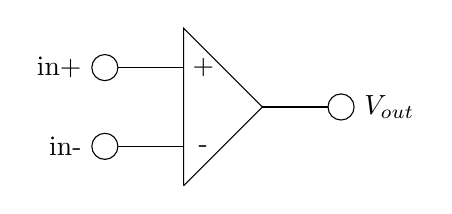
\begin{tikzpicture}
\draw (0,0) node[circle,draw=black, fill=white,radius=.1 mm, label=left:{in-}]{}
--(1,0);
\draw (0,1) node[circle,draw=black, fill=white,radius=.1 mm,label=left:{in+}]{}
--(1,1);
\draw (1,-.5)--(1,1.5)--(2,.5)--(1,-.5);
\draw (2,.5)--(3,.5) node[circle,draw=black, fill=white,radius=.1 mm, label=right:{$V_{out}$}]{};
\draw node at (1.25,1) {+};
\draw node at (1.25,0) {-};
\end{tikzpicture}
\caption{Op-amp diagram symbol. All voltages are w.r.t. reference.}
\end{center}
\end{figure}

This may seem like an odd dependent source because $V_x$ is multiplied by $\infty$. Surely that can't be\footnote{Actual operational amplifiers are not able to produce $\infty V_x$, but rather might produce \emph{only} $100000 V_x$. The consequences that this difference causes are often insignificant and aren't discussed in this book.}.\par

\begin{blevel}
Fill in the Table~\ref{T:5OP} for $V_{out}$ based on the values given for in+ and in-. Some answers might be + or - $\infty$.
\end{blevel}

\begin{table}[H]
\begin{center}
\begin{tabular}{|c|c|c|}\hline
in+&in-&$V_{out}$\\ \hline
+5V&+7V& \\ \hline
-5V&+3V& \\ \hline
-5V&-5.1V& \\ \hline
0V&0.00001V& \\ \hline
\end{tabular}
\caption{Op-amp output voltages}
\label{T:5OP}
\end{center}
\end{table}

\begin{clevel}
Explain in a sentence how to quickly determine the output of the op-amp.
\end{clevel}

\par
A real world op-amp can not produce $\infty V$ nor $-\infty V$. Worse yet, it can't do much of anything unless it is somehow provided power, usually with a positive voltage (V++) and negative voltage (V--). The op-amp then produces a max and min output voltage based on the values of positive and negative voltages supplied to it. These voltage supplies can be indicated on our diagram as such: \footnote{I will usually leave them off the drawing, but they are always there.}\\

\begin{figure}[H]
\begin{center}
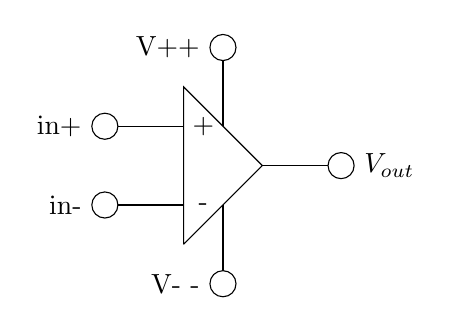
\begin{tikzpicture}
\draw (0,0) node[circle,draw=black, fill=white,radius=.1 mm, label=left:{in-}]{}
--(1,0);
\draw (0,1) node[circle,draw=black, fill=white,radius=.1 mm,label=left:{in+}]{}
--(1,1);
\draw (1,-.5)--(1,1.5)--(2,.5)--(1,-.5);
\draw (2,.5)--(3,.5) node[circle,draw=black, fill=white,radius=.1 mm, label=right:{$V_{out}$}]{};
\draw node at (1.25,1) {+};
\draw node at (1.25,0) {-};
\draw (1.5,1)--(1.5,2) node[circle,draw=black, fill=white,radius=.1 mm,label=left:{V++}]{};
\draw (1.5,0)--(1.5,-1) node[circle,draw=black, fill=white,radius=.1 mm,label=left:{V- -}]{};
\end{tikzpicture}
\caption{Op-amp with power supply connections}
\end{center}
\end{figure}

The max output voltage that the op-amp acheives can not exceed the V++ nor go below V- -.

\begin{blevel}
Fill in the Table~\ref{T:5OP2} for $V_{out}$ based on the values given for in+ and in-.
\end{blevel}

\begin{table}[H]
\begin{center}
\begin{tabular}{|c|c|c|c|c|}\hline
in+&in-&V++&V--&$V_{out}$\\ \hline
+5V&+7V&10V&-10V&-10V \\ \hline
-5V&+3V&10V&-10V& \\ \hline
-5V&-5.1V&10V&-10V& \\ \hline
0V&0.00001V&10V&-10V& \\ \hline
+5V&+7V&5V&-3V& \\ \hline
-5V&+3V&5V&-3V& \\ \hline
-5V&-5.1V&5V&-3V& \\ \hline
0V&0.00001V&5V&-3V& \\ \hline
\end{tabular}
\caption{Op-amp output values taking with known supply voltages}
\label{T:5OP2}
\end{center}
\end{table}

\begin{clevel}
Explain how to quickly determine the output of the op-amp with V++ and V-- limits.
\end{clevel}

\subsection{Feedback and Cool Tricks}
Op-amps circuits often have feedback. As a result, the idea of feedback is often introduced in introductory circuit analysis even though it applies to engineering systems in general. The following figure shows two generic engineering systems, one with feedback and one without.

\begin{figure}[H]
\begin{center}
\begin{tikzpicture}
\draw node at (-1.25,.25) {in A};
\draw node at (-1.25,1) {in B};
\draw node at (-1.25,1.75) {in C};
\draw node at (4.5,.25) {in A};
\draw node at (4.5,1) {in B};
\draw node at (1.75,1.25) {output};
\draw node at (7.75,1.25) {output};
\draw (0,0)--(0,2)--(1,2)--(1,0)--(0,0);
\draw (-1,.25)--(0,.25) (-1,1)--(0,1) (-1,1.75)--(0,1.75) (1,1)--(2,1);
\draw (6,0)--(6,2)--(7,2)--(7,0)--(6,0);
\draw (5,.25)--(6,.25) (5,1)--(6,1) (5,1.75)--(6,1.75) (7,1)--(8,1)--(8,3)--(5,3)--(5,1.75);
\end{tikzpicture}
\caption{Two engineering systems. The output of the system on the left only depends on independent inputs and has no feedback. The system on the right has feedback.}
\end{center}
\end{figure}

For systems with feedback, the output is fed back into the system as an input. To make this more clear, I'll use an example of a heating system.

\begin{figure}[H]
\begin{center}
\begin{tikzpicture}
\draw node at (-1.25,.25) {$T_A$};
\draw node at (-1.25,1) {$T_B$};
\draw node at (1,1) {$\begin{matrix}Heater\\ \text{On if $T_A>T_B$}\end{matrix}$};
\draw node at (4,1) {$\begin{matrix}Thermometer\\ \text{In room}\end{matrix}$};
\draw (0,0)--(0,2)--(2,2)--(2,0)--(0,0);
\draw (-1,.25)--(0,.25) (-1,1)--(0,1);
\draw [dashed] (2,1)--(3,1);
\draw (3,0)--(3,2)--(5,2)--(5,0)--(3,0) (5,1)--(6,1)--(6,3)--(-1,3)--(-1,1);
\end{tikzpicture}
\caption{A room heating system.}
\end{center}
\end{figure}

\begin{alevel}
Does the heating system have feedback?
\end{alevel}
\begin{alevel}
If $T_A$ is 70F and the room temp is 63F, will the heater be ON or OFF?
\end{alevel}
\begin{blevel}
In terms of $T_A$, at what temperature will the room stabilize?
\end{blevel}

Now consider the modified version of the heating system shown here.

\begin{figure}[H]
\begin{center}
\begin{tikzpicture}
\draw node at (-1.25,.25) {$T_A$};
\draw node at (-1.25,1) {$T_B$};
\draw node at (1,1) {$\begin{matrix}Heater\\ \text{On if $T_A>T_B$}\end{matrix}$};
\draw node at (4,1) {$\begin{matrix}Thermometer\\ \text{In room}\end{matrix}$};
\draw node at (3,3) {$\div 3$};
\draw (0,0)--(0,2)--(2,2)--(2,0)--(0,0);
\draw (-1,.25)--(0,.25) (-1,1)--(0,1);
\draw [dashed] (2,1)--(3,1);
\draw (3,0)--(3,2)--(5,2)--(5,0)--(3,0);
\draw [->] (5,1)--(6,1)--(6,3)--(4,3);
\draw (2,2.5)--(2,4)--(4,4)--(4,2.5)--(2,2.5);
\draw [->] (2,3)--(-1,3);
\draw (-1,3)--(-1,1);
\end{tikzpicture}
\caption{A room heating system where thermometer reading is divided by 3 before being fed back as an input.}
\end{center}
\end{figure}

\begin{alevel}
If $T_A$ is 70$^\circ$F and the room temp is 63$^\circ$F, will the heater be ON or OFF?
\end{alevel}
\begin{blevel}
In terms of $T_A$, at what temperature will the room stabilize?
\end{blevel}

\subsection{Op-amp Feedback}
Now, we're ready to look at an op-amp circuit with feedback. Consider the circuit shown in Figure~\ref{T:5OPH} shown alongside a heating system with feedback. The heating system increases the room temperature if T+ exceeds T-. The op-amp increases the output voltage if the (in+) terminal voltage exceeds the (in-)terminal voltage.
\begin{figure}[H]
\begin{center}
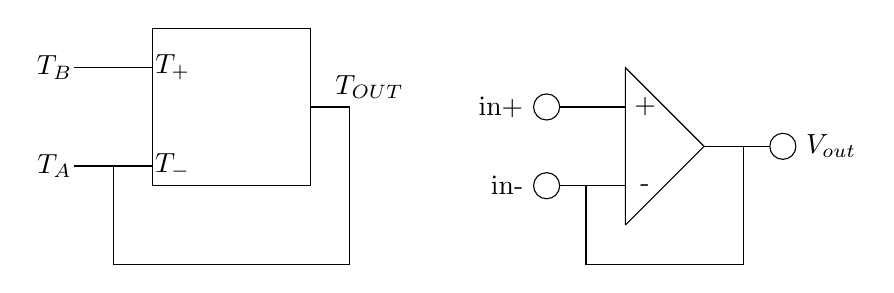
\begin{tikzpicture}
\draw node at (-6.25,.25) {$T_A$};
\draw node at (-6.25,1.5) {$T_B$};
\draw (-5,0)--(-3,0)--(-3,2)--(-5,2)--(-5,0);
\draw (-3,1)--(-2.5,1)--(-2.5,-1)--(-5.5,-1)--(-5.5,.25);
\draw (-6,.25)--(-5,.25) (-6,1.5)--(-5,1.5);
\draw node at (-4.75,1.5) {$T_{+}$};
\draw node at (-4.75,.25) {$T_{-}$};
\draw node at (-2.25,1.25) {$T_{OUT}$};

\draw (0,0) node[circle,draw=black, fill=white,radius=.1 mm, label=left:{in-}]{}
--(1,0);
\draw (0,1) node[circle,draw=black, fill=white,radius=.1 mm,label=left:{in+}]{}
--(1,1);
\draw (1,-.5)--(1,1.5)--(2,.5)--(1,-.5);
\draw (2,.5)--(3,.5) node[circle,draw=black, fill=white,radius=.1 mm, label=right:{$V_{out}$}]{};
\draw node at (1.25,1) {+};
\draw node at (1.25,0) {-};
\draw (2.5,.5)--(2.5,-1)--(.5,-1)--(.5,0);
\end{tikzpicture}
\caption{Heating system with feedback alongside op-amp with feedback.}
\label{T:5OPH}
\end{center}
\end{figure}

\begin{alevel}
Suppose $V_{out}$ were 3V and Vin+ were 5V. Would this cause Vout to increase or decrease?
\end{alevel}
\begin{blevel}
Suppose $V_{out}$ were 3V and Vin+ were 5V, then $V_{out}$ would change and eventually stabilize at what value?
\end{blevel}

Next consider a divider put into the feedback loop as shown in Figure~\ref{T:5OPH2}. The heating system output temperature must now stabilize at a value of twice $T_B$. The output voltage of the op-amp will similarly converge on a value of twice $V_{in+}$.

\begin{figure}[H]
\begin{center}
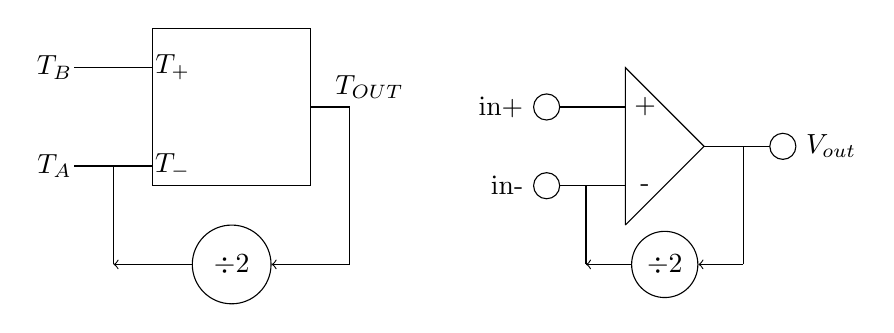
\begin{tikzpicture}
\draw node at (-6.25,.25) {$T_A$};
\draw node at (-6.25,1.5) {$T_B$};
\draw (-5,0)--(-3,0)--(-3,2)--(-5,2)--(-5,0);
\node[draw,circle,minimum size =1cm] (A) at (-4,-1){$\div 2$};
\draw [->](-2.5,-1)--(A);
\draw [->](A)-- (-5.5,-1);
\draw (-3,1)--(-2.5,1)--(-2.5,-1) (-5.5,-1)--(-5.5,.25);
\draw (-6,.25)--(-5,.25) (-6,1.5)--(-5,1.5);
\draw node at (-4.75,1.5) {$T_{+}$};
\draw node at (-4.75,.25) {$T_{-}$};
\draw node at (-2.25,1.25) {$T_{OUT}$};

\draw (0,0) node[circle,draw=black, fill=white,radius=.1 mm, label=left:{in-}]{}
--(1,0);
\draw (0,1) node[circle,draw=black, fill=white,radius=.1 mm,label=left:{in+}]{}
--(1,1);
\draw (1,-.5)--(1,1.5)--(2,.5)--(1,-.5);
\draw (2,.5)--(3,.5) node[circle,draw=black, fill=white,radius=.1 mm, label=right:{$V_{out}$}]{};
\draw node at (1.25,1) {+};
\draw node at (1.25,0) {-};
\node[draw,circle,minimum size =0.5cm] (AO) at (1.5,-1){$\div 2$};
\draw [->](2.5,-1)--(AO);
\draw [->](AO)-- (.5,-1);
\draw (2.5,.5)--(2.5,-1)(.5,-1)--(.5,0);
\end{tikzpicture}
\caption{Heating system with feedback alongside Op-amp with feedback. .}
\label{T:5OPH2}
\end{center}
\end{figure}

The next figure shows how the divide by 2 operation could be achieved using a voltage divider.

\begin{figure}[H]
\begin{center}
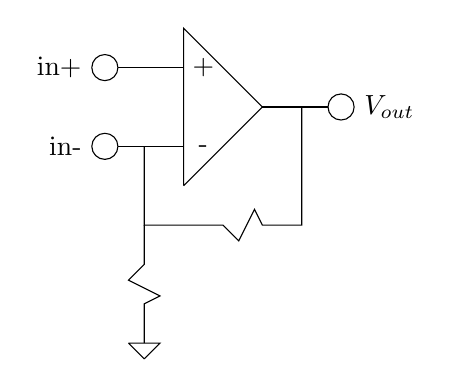
\begin{tikzpicture}
\draw (0,0) node[circle,draw=black, fill=white,radius=.1 mm, label=left:{in-}]{}
--(1,0);
\draw (0,1) node[circle,draw=black, fill=white,radius=.1 mm,label=left:{in+}]{}
--(1,1);
\draw (1,-.5)--(1,1.5)--(2,.5)--(1,-.5);
\draw (2,.5)--(3,.5) node[circle,draw=black, fill=white,radius=.1 mm, label=right:{$V_{out}$}]{};
\draw node at (1.25,1) {+};
\draw node at (1.25,0) {-};
\draw (2.5,.5)--(2.5,-1)--(2,-1)--(1.9,-.8)--(1.7,-1.2)--(1.5,-1)--(.5,-1)--(.5,0);
\draw (.5,-1)--(.5,-1.5)--(.3,-1.7)--(.7,-1.9)--(.5,-2)--(.5,-2.5);
\draw (.3,-2.5)--(.7,-2.5)--(.5,-2.7) (.3,-2.5)--(.5,-2.7);
\end{tikzpicture}
\caption{A common op-amp circuit using a voltage divider in the feedback path.}
\end{center}
\end{figure}

\begin{blevel}
Suppose the two resistors in the feedback path were the same. Further suppose Vout were 3V and Vin+ were 4V. Would this cause Vout to increase or decrease?
\end{blevel}
\begin{blevel}
Suppose the two resistors in the feedback path were the same. Suppose Vout were 3V and Vin+ were 4V. Vout would change and eventually stabilize at what value?
\end{blevel}
\begin{clevel}
Suppose the two resistors in the feedback path were labeled R1 and R2 and the voltage at Vin+ were called Vin. Determine the voltage that the output voltage would stabilize at. 
\end{clevel}

